% Copyright (C) 2014-2017 by Thomas Auzinger <thomas@auzinger.name>

\documentclass[draft,final]{vutinfth} % Remove option 'final' to obtain debug information.

% Load packages to allow in- and output of non-ASCII characters.
\usepackage{lmodern}        % Use an extension of the original Computer Modern font to minimize the use of bitmapped letters.
\usepackage[T1]{fontenc}    % Determines font encoding of the output. Font packages have to be included before this line.
\usepackage[utf8]{inputenc} % Determines encoding of the input. All input files have to use UTF8 encoding.

% Extended LaTeX functionality is enables by including packages with \usepackage{...}.
\usepackage{amsmath}    % Extended typesetting of mathematical expression.
\usepackage{amssymb}    % Provides a multitude of mathematical symbols.
\usepackage{mathtools}  % Further extensions of mathematical typesetting.
\usepackage{microtype}  % Small-scale typographic enhancements.
\usepackage[inline]{enumitem} % User control over the layout of lists (itemize, enumerate, description).
\usepackage{multirow}   % Allows table elements to span several rows.
\usepackage{booktabs}   % Improves the typesettings of tables.
\usepackage{subcaption} % Allows the use of subfigures and enables their referencing.
\usepackage[ruled,linesnumbered,algochapter]{algorithm2e} % Enables the writing of pseudo code.
\usepackage[usenames,dvipsnames,table]{xcolor} % Allows the definition and use of colors. This package has to be included before tikz.
\usepackage{nag}       % Issues warnings when best practices in writing LaTeX documents are violated.
\usepackage{todonotes} % Provides tooltip-like todo notes.
\usepackage{hyperref}  % Enables cross linking in the electronic document version. This package has to be included second to last.
\usepackage[acronym,toc]{glossaries} % Enables the generation of glossaries and lists fo acronyms. This package has to be included last.
\usepackage{paralist} %Allows usage of inline lists

% Define convenience functions to use the author name and the thesis title in the PDF document properties.
\newcommand{\authorname}{Stefan Gamerith} % The author name without titles.
\newcommand{\thesistitle}{Enrichment of Crowdsourcing Tasks with Contextual Data} % The title of the thesis. The English version should be used, if it exists.

% Set PDF document properties
\hypersetup{
    pdfpagelayout   = TwoPageRight,           % How the document is shown in PDF viewers (optional).
    linkbordercolor = {Melon},                % The color of the borders of boxes around crosslinks (optional).
    pdfauthor       = {\authorname},          % The author's name in the document properties (optional).
    pdftitle        = {\thesistitle},         % The document's title in the document properties (optional).
    pdfsubject      = {Subject},              % The document's subject in the document properties (optional).
    pdfkeywords     = {a, list, of, keywords} % The document's keywords in the document properties (optional).
}

\setpnumwidth{2.5em}        % Avoid overfull hboxes in the table of contents (see memoir manual).
\setsecnumdepth{subsection} % Enumerate subsections.

\nonzeroparskip             % Create space between paragraphs (optional).
\setlength{\parindent}{0pt} % Remove paragraph identation (optional).

\makeindex      % Use an optional index.
\makeglossaries % Use an optional glossary.
%\glstocfalse   % Remove the glossaries from the table of contents.

% Set persons with 4 arguments:
%  {title before name}{name}{title after name}{gender}
%  where both titles are optional (i.e. can be given as empty brackets {}).
\setauthor{}{\authorname}{BSc.}{male}
\setadvisor{}{Reka Marta Sabou}{MSc., PhD}{female}

% For bachelor and master theses:
%\setfirstassistant{Pretitle}{Forename Surname}{Posttitle}{male}
%\setsecondassistant{Pretitle}{Forename Surname}{Posttitle}{male}
%\setthirdassistant{Pretitle}{Forename Surname}{Posttitle}{male}

% For dissertations:
%\setfirstreviewer{Pretitle}{Forename Surname}{Posttitle}{male}
%\setsecondreviewer{Pretitle}{Forename Surname}{Posttitle}{male}

% For dissertations at the PhD School and optionally for dissertations:
% \setsecondadvisor{Pretitle}{Forename Surname}{Posttitle}{male} % Comment to remove.

% Required data.
\setaddress{Linzerstrasse 429/4215, 1140 Wien}
\setregnumber{0925081}
\setdate{01}{01}{2001} % Set date with 3 arguments: {day}{month}{year}.
\settitle{\thesistitle}{\thesistitle} % Sets English and German version of the title (both can be English or German). If your title contains commas, enclose it with additional curvy brackets (i.e., {{your title}}) or define it as a macro as done with \thesistitle.
%\setsubtitle{Optional Subtitle of the Thesis}{Optionaler Untertitel der Arbeit} % Sets English and German version of the subtitle (both can be English or German).

% Select the thesis type: bachelor / master / doctor / phd-school.
% Bachelor:
%\setthesis{bachelor}
%
% Master:
\setthesis{master}
\setmasterdegree{dipl.} % dipl. / rer.nat. / rer.soc.oec. / master
%
% Doctor:
%\setthesis{doctor}
%\setdoctordegree{rer.soc.oec.}% rer.nat. / techn. / rer.soc.oec.
%
% Doctor at the PhD School
%\setthesis{phd-school} % Deactivate non-English title pages (see below)

% For bachelor and master:
\setcurriculum{Software Engineering / Internet Computing}{Software Engineering / Internet Computing} % Sets the English and German name of the curriculum.

% For dissertations at the PhD School:
%\setfirstreviewerdata{Affiliation, Country}
%\setsecondreviewerdata{Affiliation, Country}


\begin{document}

\frontmatter % Switches to roman numbering.
% The structure of the thesis has to conform to
%  http://www.informatik.tuwien.ac.at/dekanat

\addtitlepage{naustrian} % German title page (not for dissertations at the PhD School).
\addtitlepage{english} % English title page.
\addstatementpage

\begin{danksagung*}
\todo{Ihr Text hier.}
\end{danksagung*}

\begin{acknowledgements*}
\todo{Enter your text here.}
\end{acknowledgements*}

\begin{kurzfassung}
\todo{Ihr Text hier.}
\end{kurzfassung}

\begin{abstract}
\todo{Enter your text here.}
\end{abstract}

% Select the language of the thesis, e.g., english or naustrian.
\selectlanguage{english}

% Add a table of contents (toc).
\tableofcontents % Starred version, i.e., \tableofcontents*, removes the self-entry.

% Switch to arabic numbering and start the enumeration of chapters in the table of content.
\mainmatter



\chapter{Introduction}
\todo{Enter your text here.}
\section{Motivation}
\todo{Enter your text here.}
\section{Aim of the Work (e.g. Research Questions)}
\todo{Enter your text here.}
\section{Contributions}
\todo{Enter your text here.}
\section{Structure of the Work}
\todo{Enter your text here.}



\chapter{State of the Art}
\todo{Enter your text here.}
\section{Crowdsourcing}
\todo{Enter your text here.}
\section{Crowdsourcing in the Semantic Web}
\todo{Enter your text here.}
\section{The uComp Protege Plugin}
\todo{Enter your text here.}
\section{Enrichment of crowdsourcing tasks with contextual data}
\todo{Enter your text here.}



\chapter{Methodology}
\todo{Enter your text here.}



\chapter{Context Enrichment Methods}\label{chap:context_enrichment_methods}
While in~\hyperref[chap:implementation]{Chapter~\ref*{chap:implementation}} the technical foundation for implementing the Context Enrichment Methods was built, this Chapter describes these on a more conceptual level. There was no limitation on the used settings or data. Instead, the context used for ontology validation was created from general purpose internal and external sources. 

First, \hyperref[sec:neighboring_nodes]{Section~\ref*{sec:neighboring_nodes}} introduces a novel Context Enrichment Method which takes neighboring nodes~(i.e. subclass relations) into account. Second, a method of embedded context using metadata is discussed in \hyperref[sec:embedded_context]{Section~\ref*{sec:embedded_context}} and last, \hyperref[sec:external_source]{Section~\ref*{sec:external_source}} contains Context Enrichment using data from external sources.
\section{Neighboring Nodes}\label{sec:neighboring_nodes}
This Section starts with an conceptual overview of how neighboring nodes in an ontology graph are used to generate contextual information for ontology validation. Then, existing approaches on generating textual definitions for an ontology are examined. As in the literature~\cite{soton265735} the term \textit{ontology verbalisation} is commonly used as a short-term for that task, it is used in the remainder of this Section. We conclude that even though that there exists the major tool \textit{OWL Verbalizer}\footnote{\url{http://mcs.open.ac.uk/nlg/SWAT/Verbaliser.html} accessed 2018/04/30} which transforms a generic OWL~ontology into english sentences, we could not integrate it into Context Enrichment process because 
\begin{inparaenum}[a)]
		\item it was designed as a standalone tool written in SWI-Prolog\footnote{\url{http://www.swi-prolog.org/} accessed 2018/04/30} and
		\item as input it only accepts the whole OWL~ontology 
\end{inparaenum}.
However, to make concept definitions and relations more understandable for non-experts, some revised rules were integrated in our enrichment process.

To illustrate the concept of neighboring nodes and how they relate to the Context Enrichment approach explained later, a simple ontology graph is given in~\hyperref[fig:simple_owl_graph]{Figure~\ref*{fig:simple_owl_graph}} describing the teacher/pupil domain.
\begin{figure}
	 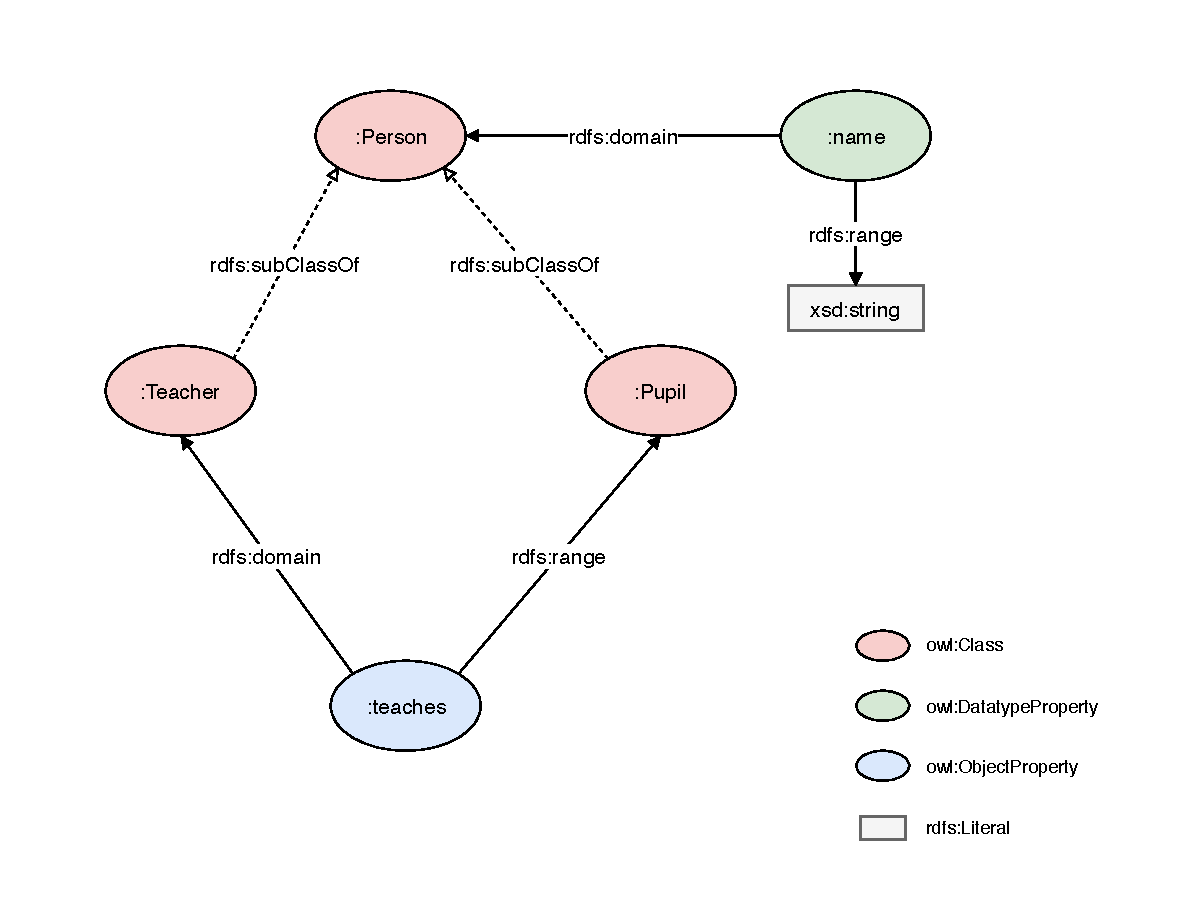
\includegraphics[width=\textwidth]{drawio/University_Ontology_Example}
	 \caption{Simple OWL ontology graph}\label{fig:simple_owl_graph}
\end{figure}
For example, if the concept \textit{:Teacher} is taken as reference node, it makes sense to not only consider the concept itself, but instead include connected nodes~(e.g. the concept \textit{:Person} and the object property \textit{:teaches}) in the enrichment process. 

As in the guidelines for conducting crowdsourcing research~\cite{sarasua2015crowdsourcing} emerged from empirical studies, the authors recommended to avoid technical terms in crowdsourcing questions. To facilitate this need, we examined an existing approach on ontology verbalisation and how they could be integrated in the Context Enrichment process. 


\section{Embedded Context}\label{sec:embedded_context}
%Get concept definition from wordnik
\section{External Source}\label{sec:external_source}
%On medical ontology which already has some definitions; collaboratively edited;


\chapter{Experimental Evaluation}
Initial paper~\cite{liu2005semi} for evaluation data using ontology learning techniques.
\todo{Enter your text here.}


\chapter{Implementation}\label{chap:implementation}
%Include also methods for spam detection
\section{Environment}
\section{Conceptual Architecture}




\chapter{Evaluation of the code}
\todo{Enter your text here.}
\section{Code Quality Assurance}
\todo{Enter your text here.}
\section{Background}
\todo{Enter your text here.}
\section{Quality Metrics}
\todo{Enter your text here.}
\section{Quality Evaluation}
\todo{Enter your text here.}



\chapter{Results}
\todo{Enter your text here.}



\chapter{Discussion \& Conclusion}
\todo{Enter your text here.}
%Revisit Research Questions here



\chapter{Summary \& Future Work}
\todo{Enter your text here.}



\backmatter

% Use an optional list of figures.
\listoffigures % Starred version, i.e., \listoffigures*, removes the toc entry.

% Use an optional list of tables.
\cleardoublepage % Start list of tables on the next empty right hand page.
\listoftables % Starred version, i.e., \listoftables*, removes the toc entry.

% Use an optional list of alogrithms.
%\listofalgorithms
%\addcontentsline{toc}{chapter}{List of Algorithms}

% Add an index.
%\printindex

% Add a glossary.
%\printglossaries

% Add a bibliography.
\bibliographystyle{alpha}
\bibliography{literature}

\end{document}